\section{Support Vector Machine (SVM)} \label{sec:prob2}
In this section, we consider the Support Vector Machine (SVM) for binary classification of several 2D datasets.

\subsection{Part 1}
We implemented the dual form of a linear SVM with slack variables. I first converted the input data into a standard format, then we used the cvxopt Python package to execute the quadratic programming to find the desired $\alpha$ values.

The inputs to the cvxopt solver were:
\begin{itemize}
	\item $P \in \Re^{n x n}$, where $P[i,j] = Y[i]Y[j]K(X[i],X[j])$
	\item $q = [-1, -1, ...] \in \Re^n$
	\item $G = [-I, I]^T \in \Re^{2n x n}$
	\item $h = [0, 0, ...; C, C, ...]$
	\item $A = Y^T$
	\item $b=0$
\end{itemize}

With the simple 4 element dataset $\{((2,2),+1),((2,3),+1),((0,-1),-1),((-3,-2),-1)\}$, the algorithm outputs $(2,2)$ and $(0,-1)$ as the support vectors, meaning they lie on the boundaries of the margin, seen in~\cref{fig:2_1_decisions}.
The weight vector has elements $w = [0.308, 0.462]$ and bias, $b = -0.538$.
The training error is zero for this simple dataset.
We use regularization term $C=1$ for all results in this and the next subsection.

\begin{figure}
	\centering
	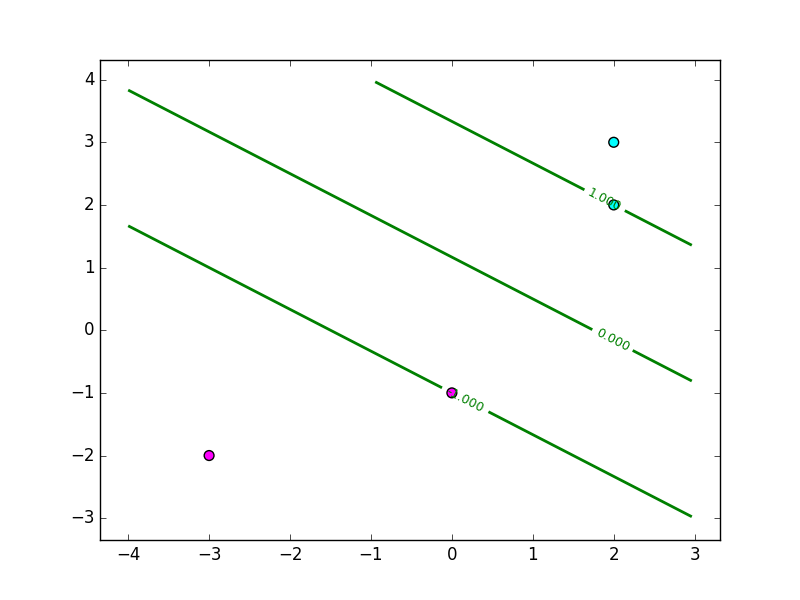
\includegraphics [trim=0 0 0 0, clip, angle=0, width=0.8\columnwidth,
	keepaspectratio]{figures/2_1_decisions}
	\caption{Simple 4-element dataset (positive elements in cyan, negative in magenta) is separated by SVM. The three lines are the decision boundary ($\hat{y}=0.0$) and positive and negative margin boundaries ($\hat{y}=\pm1.0$) and two elements (support vectors) lie directly on boundaries of margin. Training error is zero.}
	\label{fig:2_1_decisions} 
\end{figure}

\subsection{Part 2}
Next, we used SVM to classify data from four much larger 2D datasets.
The weights and bias of the decision boundary are generated using the training data, shown on the top row of~\cref{fig:2_2_decisions}, and then tested on the validation set shown in the bottom row of the same figure.
Each column represents one dataset, presumably from the same distribution but with slightly different data.
The leftmost dataset is easiest to linearly separate, whereas the middle two datasets have significant overlap between classes in this feature space.
The rightmost dataset is not well-suited for a linear classifier because the data seems to have four distinct clusters at opposite ends of a rectangle.

The classification accuracy on the validation set matches the intuition from the plots. The first and third datasets are classified most accurately, while the fourth dataset is essentially equivalent to a random coinflip.
For three of the four datasets, the training accuracy is at least as high as the validation accuracy.
This is expected, because the model typically performs worse on data that was not seen during testing.
In these cases, though, the accuracy difference is very minor.

\begin{table}[ht!]
\centering
\begin{tabular}{||c c c||}  
 \hline
 Dataset & Training Accuracy (\%) & Training Accuracy (\%) \\ [0.5ex] 
 \hline\hline
 1 & 100.0 & 100.0 \\ 
 \hline
 2 & 82.75 & 84.0 \\
 \hline
 3 & 98.75 & 96.5 \\
 \hline
 4 & 51.0 & 48.5 \\
 \hline
\end{tabular}
\caption{Accuracy of linear SVM on four datasets in~\cref{fig:2_2_decisions}.}
\label{table_svm_2_2}
\end{table}

\begin{figure}
	\centering
	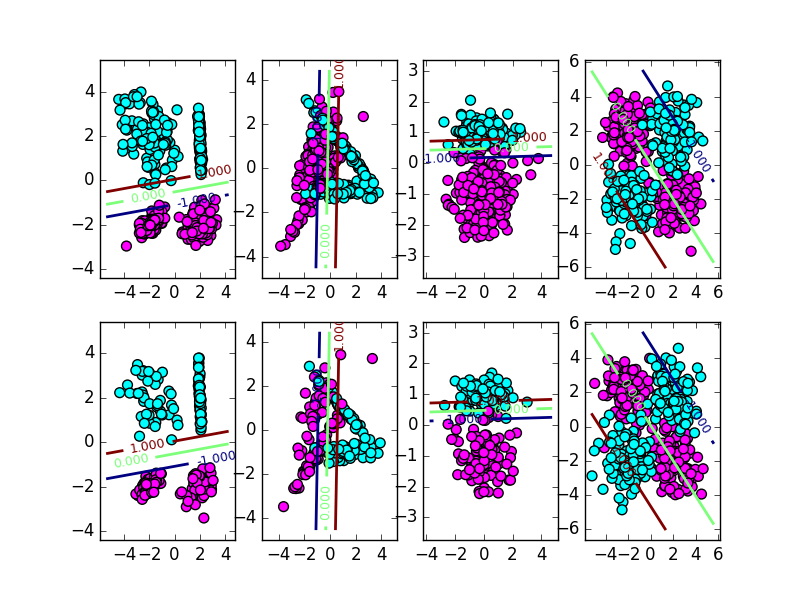
\includegraphics [trim=0 0 0 0, clip, angle=0, width=0.8\columnwidth,
	keepaspectratio]{figures/2_2_decisions}
	\caption{Four 2D datasets (positive elements in cyan, negative in magenta) are separated by SVM. The top row is the four training datasets, and the bottom row is the four corresponding validation sets.
	The three lines are the decision boundary ($\hat{y}=0.0$ in green) and positive and negative margin boundaries ($\hat{y}=\pm1.0$ in red/blue).}
	\label{fig:2_2_decisions} 
\end{figure}

\subsection{Part 3}
Next, we add an ability to handle kernel functions to the dual SVM implementation.
Two kernels are considered: linear kernel ($K(x,x')=x^T\cdot x$) and gaussian RBF kernel ($K(x,x')=exp(-\gamma||w-w'||^2$).
The regularization parameter, C, was set to 1 in previous sections, but here we are interested in how its value affects the results.

The decision boundaries with the two kernels on the four datasets are shown in~\cref{fig:2_3_decisions}.
The left two datasets can be separated pretty well by a linear kernel (top row), and while the Gaussian RBF (bottom row) can be tuned to classify reasonably well, but not to an extent that is worth the extra computational cost.
The rightmost dataset shows a clear example of a linear kernel failing where a gaussian RBF kernel shines.
The data is not linearly separable in the original feature space, so the linear kernel's accuracy is about as bad as guessing.
The Gaussian RBF kernel encloses the four clusters and classifies accurately.
It could be argued that this decision boundary overfits the data, especially clear around the edges of the boundaries.
The C parameter could be tuned to adjust this effect, but the computation time involved is significant.
The bandwidth parameter, $\gamma$ was adjusted for each dataset to get this performance (0.01 for the left two plots, 1.0 for the right two), and this parameter affects the spread of the kernel.


On the left of~\cref{fig:2_3_margin_sv}, the geometric margin ($1/||w||$) decreases as C increases in general.
These results are shown for each of the four datasets, for the two kernel functions, so there are 8 curves.
In one case, the margin increases after an increase in C.
It makes sense that margin would generally decrease with an increase in C, because more penalty is being applied to incorrectly classified samples, and therefore $||w||$ will increase to overfit the dataset slightly more and reduce the number of incorrectly classified samples.

On the right of~\cref{fig:2_3_margin_sv}, a similar concept applies to the number of support vectors as C increases.
Any sample with non-zero $\alpha_i$ is a support vector, including mis-classified samples, and with small C, the penalty of having many support vectors is low. As C increases, the margin shrinks and the number of support vectors decreases.

Maximizing the geometric margin on the training set is not an appropriate criterion for selecting C because that method will simply choose the weights corresponding to C=0.
This eliminates any allowance of slack, where misclassified points can be ignored to improve the model's ability to generalize.
An alternative method to choose C is to train many different SVM classifiers with different C values, and evaluate the classification accuracy on a validation set.
Then, choose the value of C that corresponds to high accuracy.


\begin{figure}
	\centering
	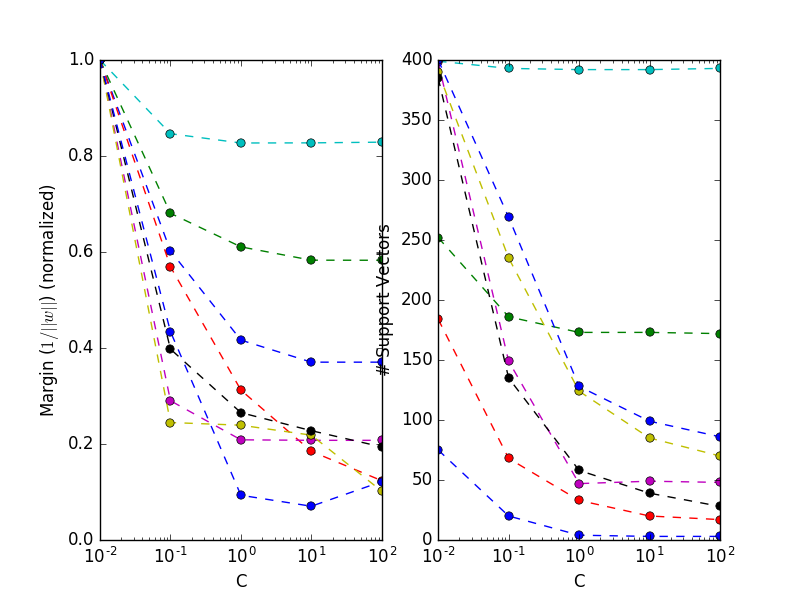
\includegraphics [trim=0 0 0 0, clip, angle=0, width=0.8\columnwidth,
	keepaspectratio]{figures/2_3_margin_sv}
	\caption{For each of four datasets, and for each of two kernel functions, on the right, the margin is plotted against regularization paramter C. As C increases, generally margin decreases. The margins are normalized by their value when $C=10^{-2}$. On the left, the number of support vectors decreases as C increases.}
	\label{fig:2_3_margin_sv} 
\end{figure}

\begin{figure}
	\centering
	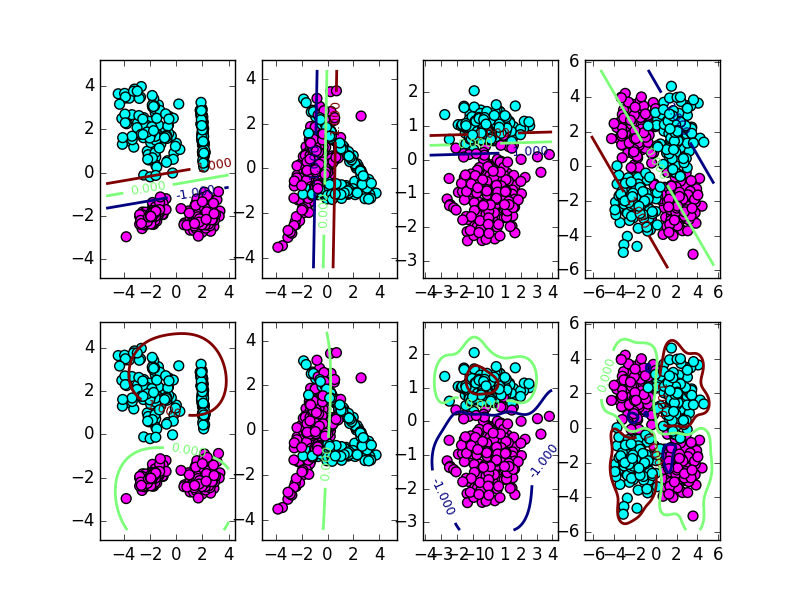
\includegraphics [trim=0 0 0 0, clip, angle=0, width=0.8\columnwidth,
	keepaspectratio]{figures/2_3_decisions}
	\caption{Each column is one validation set, with the top row showing the SVM decision boundary using a linear kernel, and the bottom row using a Gaussian RBF kernel. The Gaussian RBF can generate curved decision boundaries which is necessary for the rightmost dataset. The left datasets can be accurately/simply classified with a linear kernel, which is also less computationally intensive.}
	\label{fig:2_3_decisions} 
\end{figure}

